\documentclass[conference]{IEEEtran}

\usepackage{graphicx}
\usepackage{amsmath}
\usepackage{booktabs}
\usepackage{array}
\usepackage{url}

\title{Simulation-Based Implementation of Lean Manufacturing Techniques for Productivity Improvement: A Data-Driven Case Study From a Beverage Bottling Line}

\author{
\IEEEauthorblockN{Divash Krishnam, Ashutosh Verma, Raja}
\IEEEauthorblockA{Department of Production and Industrial Engineering\\
India\\
Email: add-your-email-before-submission}
\and
\IEEEauthorblockN{Guide}
\IEEEauthorblockA{Dr.\ MOHD SHUAIB\\
Mechanical Department\\
India}
}

\begin{document}

\maketitle

\begin{abstract}
Lean manufacturing is widely recognized as an effective strategy for reducing waste and improving productivity, yet many small and medium-sized manufacturing firms still face difficulty in deciding which lean techniques should be implemented first. This challenge becomes more serious when the firm has limited resources and cannot afford repeated trial-and-error interventions on the shop floor. This paper develops a self-contained, data-driven framework to evaluate lean interventions using a real industrial production dataset from a beverage bottling line monitored through an Industrial Internet of Things system. The dataset contains 59 production summary records across 56 calendar production days between July 22, 2022 and February 6, 2023, 265 hourly operating observations, and 1,388 downtime events. The study first analyzes throughput, operating time, pause time, product mix, and temporal efficiency variation. Next, the downtime structure is examined by classifying events into micro-, minor-, and major-stoppage categories. Finally, an event-level bootstrap simulation with 5,000 replications is used to compare three lean scenarios: 5S with visual management, total productive maintenance, and an integrated lean bundle. The observed system produced 212,358 liters with an overall availability of 42.66\%. Downtime analysis shows that micro-stoppages represent 61.31\% of all events but only 13.59\% of downtime minutes, whereas major stoppages represent 6.77\% of events but consume 66.26\% of lost time. Simulation results show that 5S and visual management improve output by 2.33\%, total productive maintenance improves output by 20.61\%, and the integrated lean bundle improves output by 32.19\%, while increasing simulated availability from 42.37\% to 55.33\%. The findings indicate that maintenance-led reduction of major stoppages should be prioritized before broader workplace-organization efforts when downtime severity is highly concentrated.
\end{abstract}

\begin{IEEEkeywords}
Lean manufacturing, productivity improvement, discrete-event simulation, downtime analysis, total productive maintenance, 5S, bottling line, SMEs, IIoT.
\end{IEEEkeywords}

\section{Introduction}
Lean manufacturing continues to be one of the most influential improvement philosophies in production engineering because it targets waste elimination, flow stabilization, quality improvement, and better resource utilization. In practice, however, the major problem is not whether lean tools are useful, but which tool should be implemented first. For small and medium-sized enterprises, a poor implementation sequence can consume scarce time and resources without delivering meaningful productivity gains.

Simulation is highly valuable in this context because it allows engineers to test alternative improvement plans before altering the real manufacturing system. Prior studies have shown that lean tools can improve manufacturing performance, but their effect depends on the nature of the system losses and the implementation context [1], [4], [5]. At the same time, the growing connection between lean and digital manufacturing suggests that event-level production data can support more precise lean decision-making [6], [10].

This paper addresses that opportunity by using an open industrial dataset from a beverage bottling line [8]. The dataset is especially suitable for lean analysis because it combines production summaries, hourly operating records, and detailed downtime-event data gathered through an IIoT-based monitoring system [7]. Using these data, the present study develops a reproducible simulation-based lean evaluation framework.

The contributions of the paper are fourfold:
\begin{enumerate}
    \item it translates real industrial data into a lean-analysis workflow;
    \item it quantifies the difference between downtime frequency and downtime severity;
    \item it compares alternative lean interventions through simulation rather than intuition alone; and
    \item it provides a reusable case-study structure for final-year research and SME-oriented manufacturing analysis.
\end{enumerate}

\section{Literature Review and Research Gap}
Belekoukias \emph{et al.} [1] showed that lean tools can improve operational performance, but they also noted that performance improvement depends strongly on context. Oleghe and Salonitis [2] argued that lean evaluation still requires stronger quantitative modeling, especially where dynamic process behavior and human interaction affect production stability.

Simulation has become one of the most useful methods for bridging that gap. Yu and Chen [3] reviewed factory simulation in SMEs and concluded that simulation offers strong decision-support value but remains underused in smaller firms because accessible and transferable applications are limited. Possik \emph{et al.} [4] proposed a co-simulation framework for evaluating lean techniques and showed that different tools have different leverage depending on the system structure. Frecassetti \emph{et al.} [5] demonstrated that simulation can support the introduction of lean practices in an SME by comparing alternative interventions before implementation.

Digital manufacturing research has further strengthened this direction. Bokhorst \emph{et al.} [6] found that smart manufacturing often builds directly on lean principles. Reslan \emph{et al.} [10] showed that digital twins can strengthen value stream mapping and improve lean diagnosis. In food and beverage SMEs, Matindana and Shoshiwa [9] found that lean implementation is relevant, but quantitative event-driven case studies are still relatively limited.

Three gaps emerge from the literature:
\begin{enumerate}
    \item many lean-simulation studies use proprietary industrial data and are difficult to reproduce;
    \item many studies discuss lean conceptually without linking event-level downtime data to scenario-based simulation; and
    \item SME-relevant manufacturing sectors such as food and beverage still have comparatively fewer open, data-driven lean case studies.
\end{enumerate}

This paper addresses these gaps by combining open industrial data, downtime-event analysis, and simulation-based lean evaluation in one self-contained study.

\section{Problem Formulation}
The production line studied in this paper experiences high variability in downtime and operating performance. The main research problem is to determine which lean strategy should be given priority to maximize productivity improvement under real operating conditions.

The main performance relationships used are:
\begin{equation}
A = \frac{T_{op}}{T_{mon}}
\end{equation}
where $A$ is operational availability, $T_{op}$ is operating time, and $T_{mon}$ is monitored time.

\begin{equation}
T_{dt} = T_{mon} - T_{op}
\end{equation}
where $T_{dt}$ is downtime.

\begin{equation}
R = \frac{Q}{T_{op}}
\end{equation}
where $Q$ is output in liters and $R$ is liters produced per operating hour.

\begin{equation}
Q' = R(T_{mon} - T'_{dt})
\end{equation}
where $Q'$ is simulated output under an improvement scenario and $T'_{dt}$ is scenario-adjusted downtime.

\begin{equation}
\%\Delta Q = \frac{Q' - Q}{Q} \times 100
\end{equation}

\section{Dataset and Methodology}
\subsection{Dataset}
The study uses the \emph{Industrial Production Time-Series Dataset from a Beverage Bottling Line} published on Zenodo on January 4, 2026 [8]. The monitoring period covers July 22, 2022 to February 6, 2023. The dataset contains 59 production summary records, 56 calendar production days, 265 hourly operating observations, and 1,388 downtime events. The observed products are 3-liter and 5-liter containers.

\begin{table}[!t]
\caption{Dataset Characteristics}
\centering
\begin{tabular}{lr}
\toprule
Attribute & Value \\
\midrule
Production summary records & 59 \\
Calendar production days & 56 \\
Hourly operating observations & 265 \\
Downtime events & 1,388 \\
Total liters produced & 212,358 \\
Total units produced & 60,888 \\
Total monitored time & 238.65 h \\
Total operating time & 101.81 h \\
\bottomrule
\end{tabular}
\end{table}

\subsection{Analytical Steps}
The methodology followed six steps:
\begin{enumerate}
    \item data extraction and cleaning;
    \item baseline productivity and downtime analysis;
    \item downtime classification into micro, minor, and major stoppages;
    \item day-level production-rate estimation;
    \item event-level bootstrap simulation with 5,000 replications; and
    \item scenario comparison using output, efficiency, and pause-time reduction.
\end{enumerate}

Downtime categories were defined as follows:
\begin{itemize}
    \item micro-stoppages: $t \leq 2$ min,
    \item minor stoppages: $2 < t \leq 10$ min,
    \item major stoppages: $t > 10$ min.
\end{itemize}

Three improvement scenarios were tested:
\begin{enumerate}
    \item 5S + Visual Management: 15\% of micro-stoppages eliminated;
    \item Total Productive Maintenance: 25\% reduction in major stoppage duration;
    \item Integrated Lean Bundle: 20\% of micro-stoppages eliminated, 15\% reduction in minor stoppages, and 30\% reduction in major stoppages.
\end{enumerate}

\subsection{Algorithmic Logic}
The model uses a data-driven bootstrap simulation. First, daily production and downtime records are converted into baseline operating profiles. Second, these observed day profiles are resampled with replacement across 5,000 replications to preserve real production variability. Third, lean rules are applied to the sampled downtime events. Finally, pause time, operating time, availability, and output are recalculated.

In practical terms, the algorithm repeatedly asks: if the observed downtime pattern is improved by a specific lean intervention, how much output is recovered?

\subsection{How Lean Manufacturing Was Applied to the Data}
Lean manufacturing was applied directly to the downtime data by mapping each lean tool to a specific loss category. 5S and visual management were linked to micro-stoppages, because better organization and visual control mainly reduce small avoidable interruptions. Total productive maintenance was linked to major stoppages, because improved maintenance reduces severe breakdown duration. The integrated lean bundle was linked to all three stoppage classes. In this way, lean was used as a rule-based transformation of measured production losses rather than only as a theoretical concept.

\section{Results}
\subsection{Baseline Performance}
The observed production system produced 212,358 liters from 60,888 units during 238.65 monitored hours. Effective operating time was only 101.81 hours, while pause time reached 137.56 hours, producing an overall observed availability of 42.66\%.

\begin{table}[!t]
\caption{Baseline Performance Indicators}
\centering
\begin{tabular}{lr}
\toprule
Metric & Value \\
\midrule
Total production & 212,358 L \\
Total units produced & 60,888 \\
Monitored time & 238.65 h \\
Operating time & 101.81 h \\
Pause time & 137.56 h \\
Observed availability & 42.66\% \\
\bottomrule
\end{tabular}
\end{table}

\begin{figure}[!t]
\centering
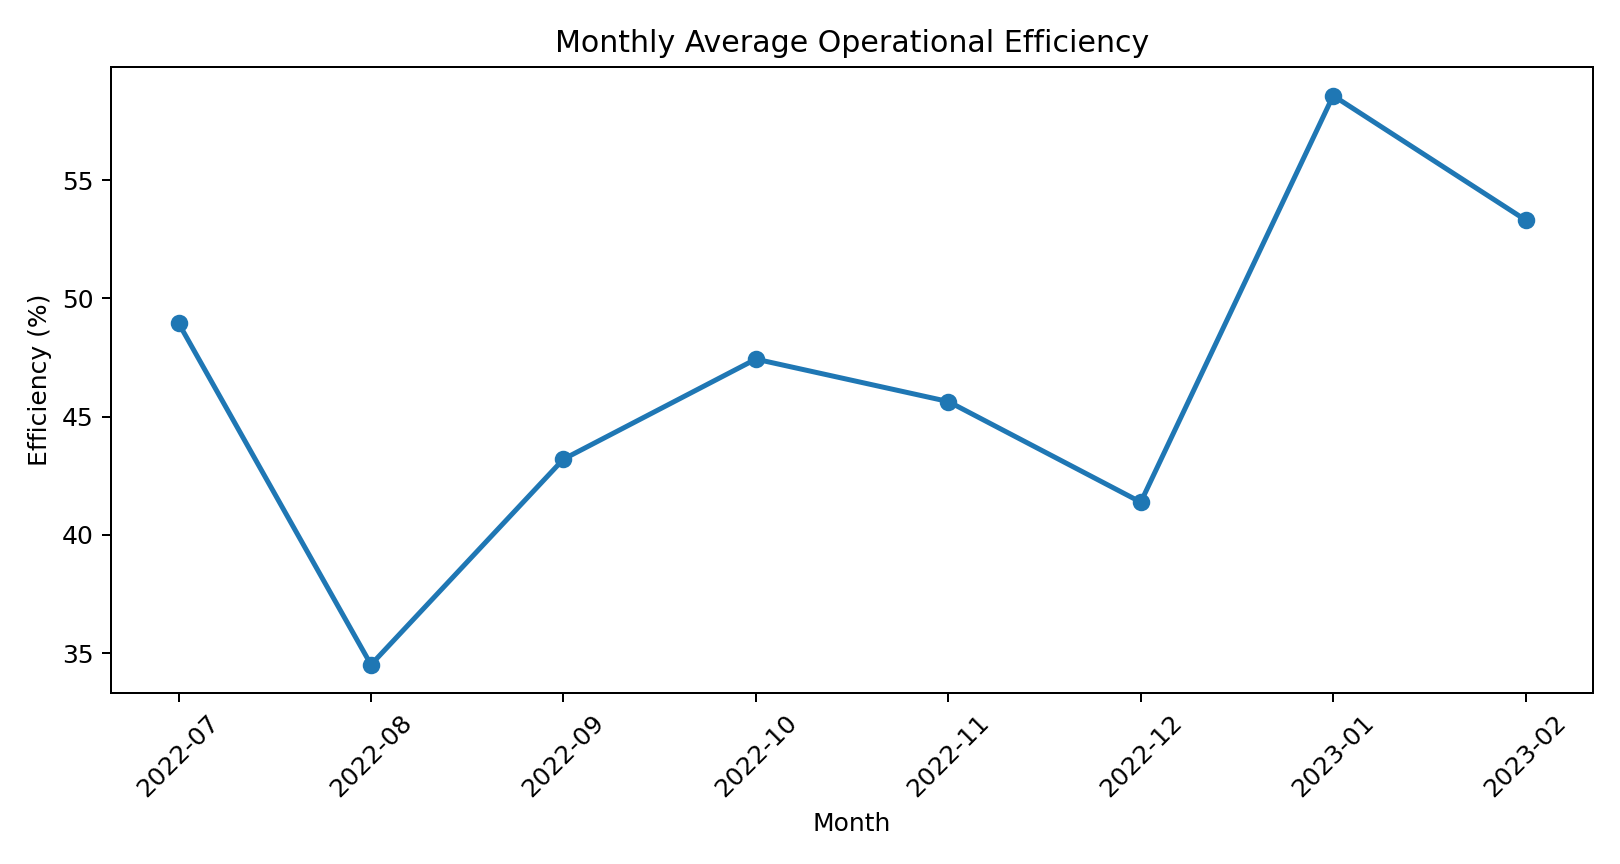
\includegraphics[width=\columnwidth]{outputs/monthly_efficiency.png}
\caption{Monthly average operational efficiency from the real dataset.}
\end{figure}

\subsection{Downtime Structure}
The downtime distribution is heavily right-skewed. The median event duration is 1.50 min, the 90th percentile is 6.50 min, the 95th percentile is 13.74 min, and the maximum event duration is 349.83 min.

\begin{table}[!t]
\caption{Downtime Category Structure}
\centering
\begin{tabular}{lrr}
\toprule
Category & Event Count & Share of Downtime Minutes \\
\midrule
Micro ($\leq$ 2 min) & 851 & 13.59\% \\
Minor (2--10 min) & 443 & 20.15\% \\
Major ($>$ 10 min) & 94 & 66.26\% \\
\bottomrule
\end{tabular}
\end{table}

\begin{figure}[!t]
\centering
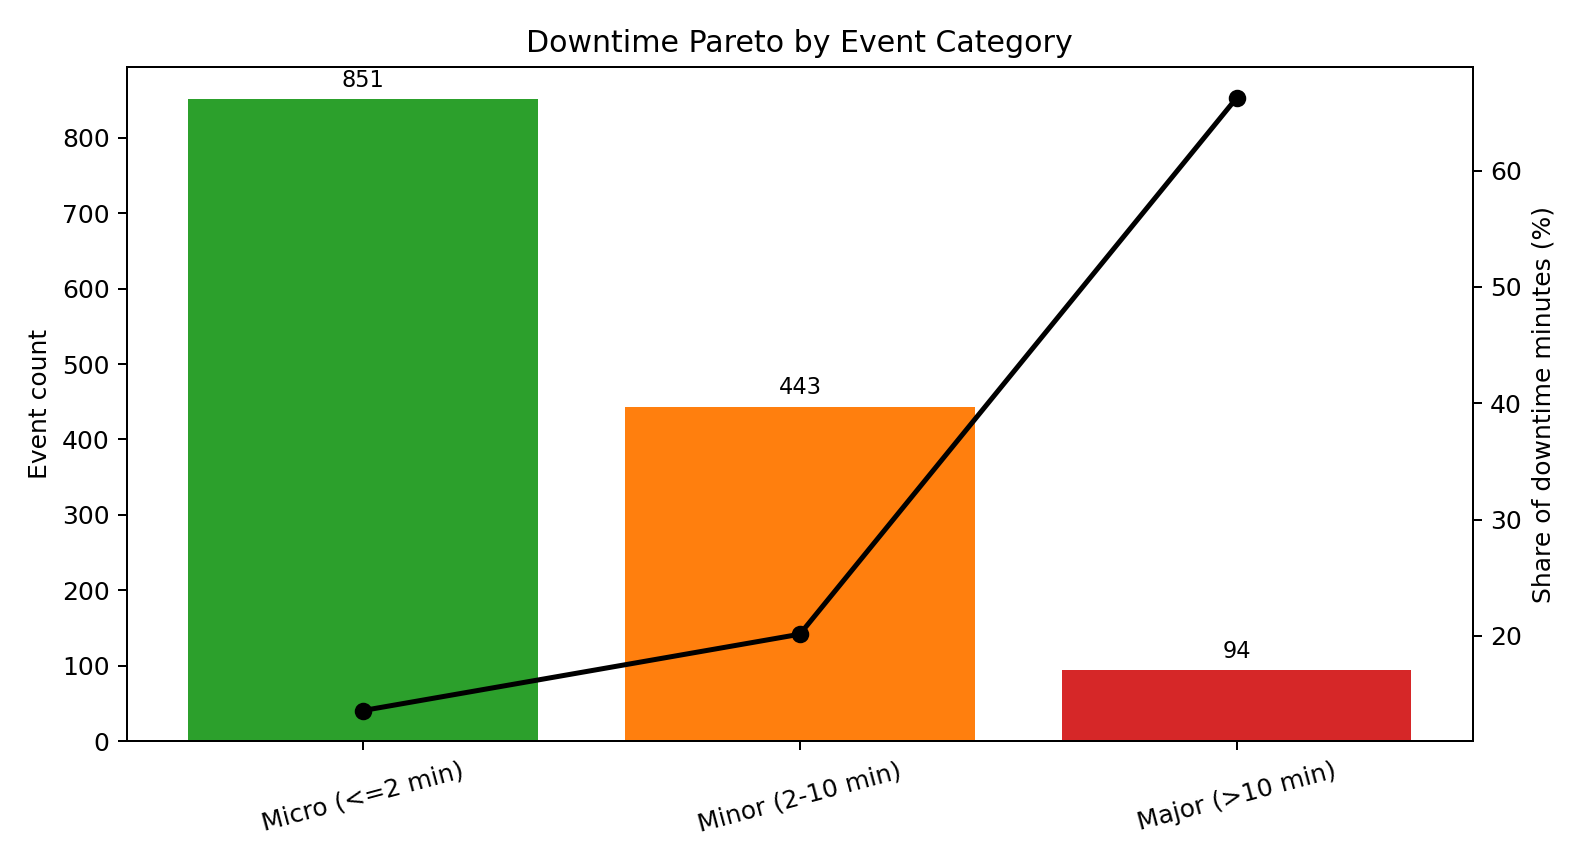
\includegraphics[width=\columnwidth]{outputs/downtime_category_pareto.png}
\caption{Downtime Pareto by event category.}
\end{figure}

Micro-stoppages account for 61.31\% of all events but only 13.59\% of total downtime minutes. Major stoppages account for just 6.77\% of events but consume 66.26\% of lost time. This difference explains why high-severity downtime should receive greater priority than high-frequency downtime.

\begin{figure}[!t]
\centering
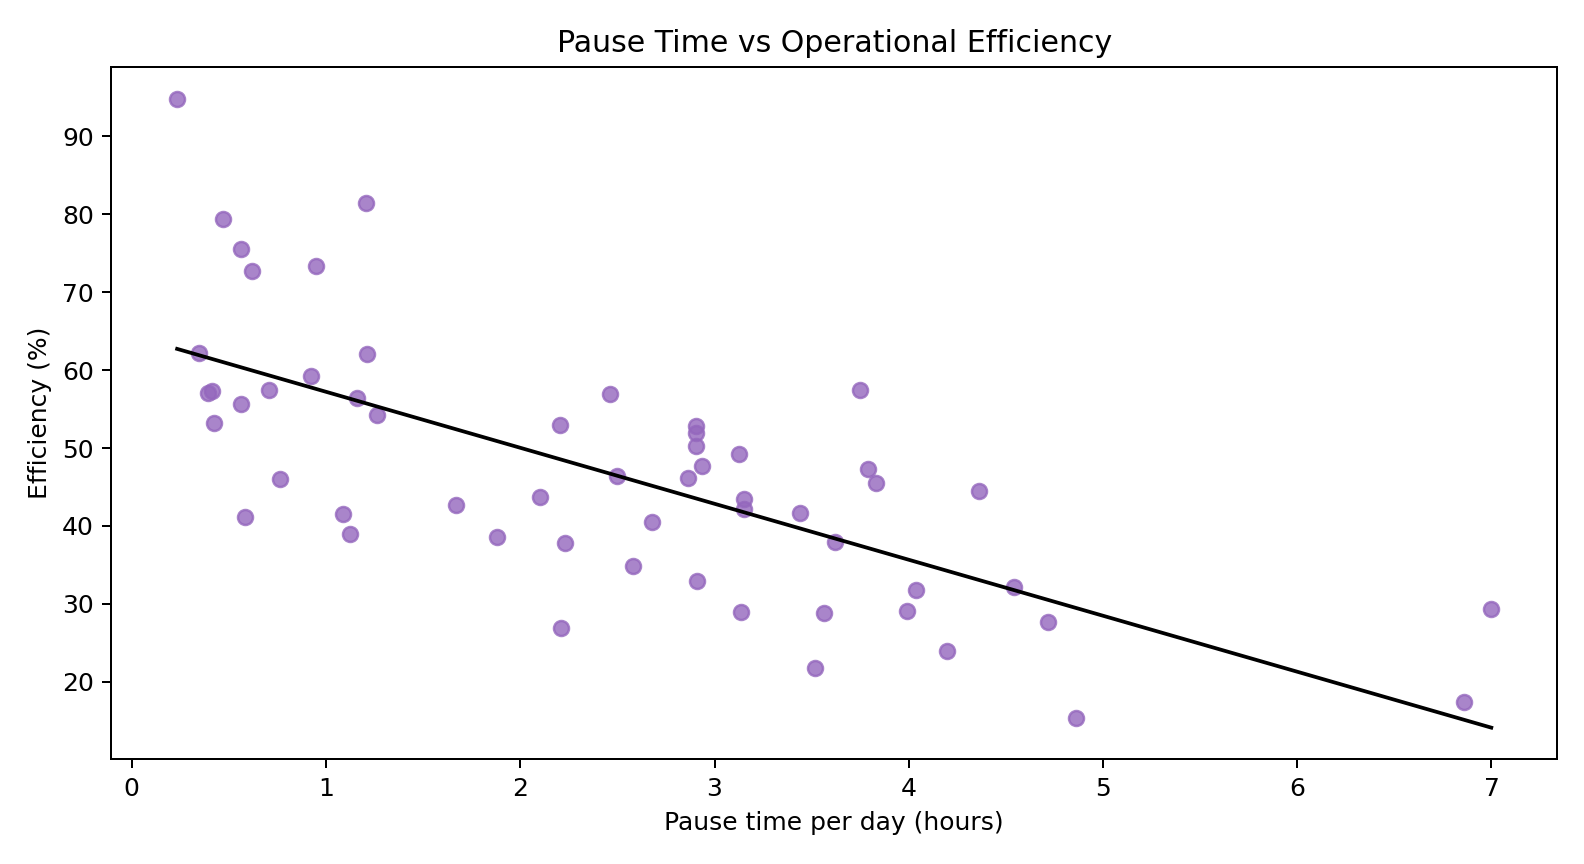
\includegraphics[width=\columnwidth]{outputs/pause_vs_efficiency.png}
\caption{Daily pause time versus operational efficiency.}
\end{figure}

\subsection{Simulation Results}
The simulation baseline produced 211,924.69 liters on average across the resampled production horizon, which closely matches the observed output of the plant. The scenario results are shown in Table III.

\begin{table}[!t]
\caption{Simulation Results for Lean Scenarios}
\centering
\begin{tabular}{lrrrr}
\toprule
Scenario & Output (L) & Gain (\%) & Eff. (\%) & Gain (pp) \\
\midrule
Baseline & 211,924.69 & 0.00 & 42.37 & 0.00 \\
5S + Visual Mgmt. & 216,866.69 & 2.33 & 43.25 & 0.88 \\
TPM & 255,604.10 & 20.61 & 50.81 & 8.44 \\
Integrated Bundle & 280,142.22 & 32.19 & 55.33 & 12.96 \\
\bottomrule
\end{tabular}
\end{table}

\begin{figure}[!t]
\centering
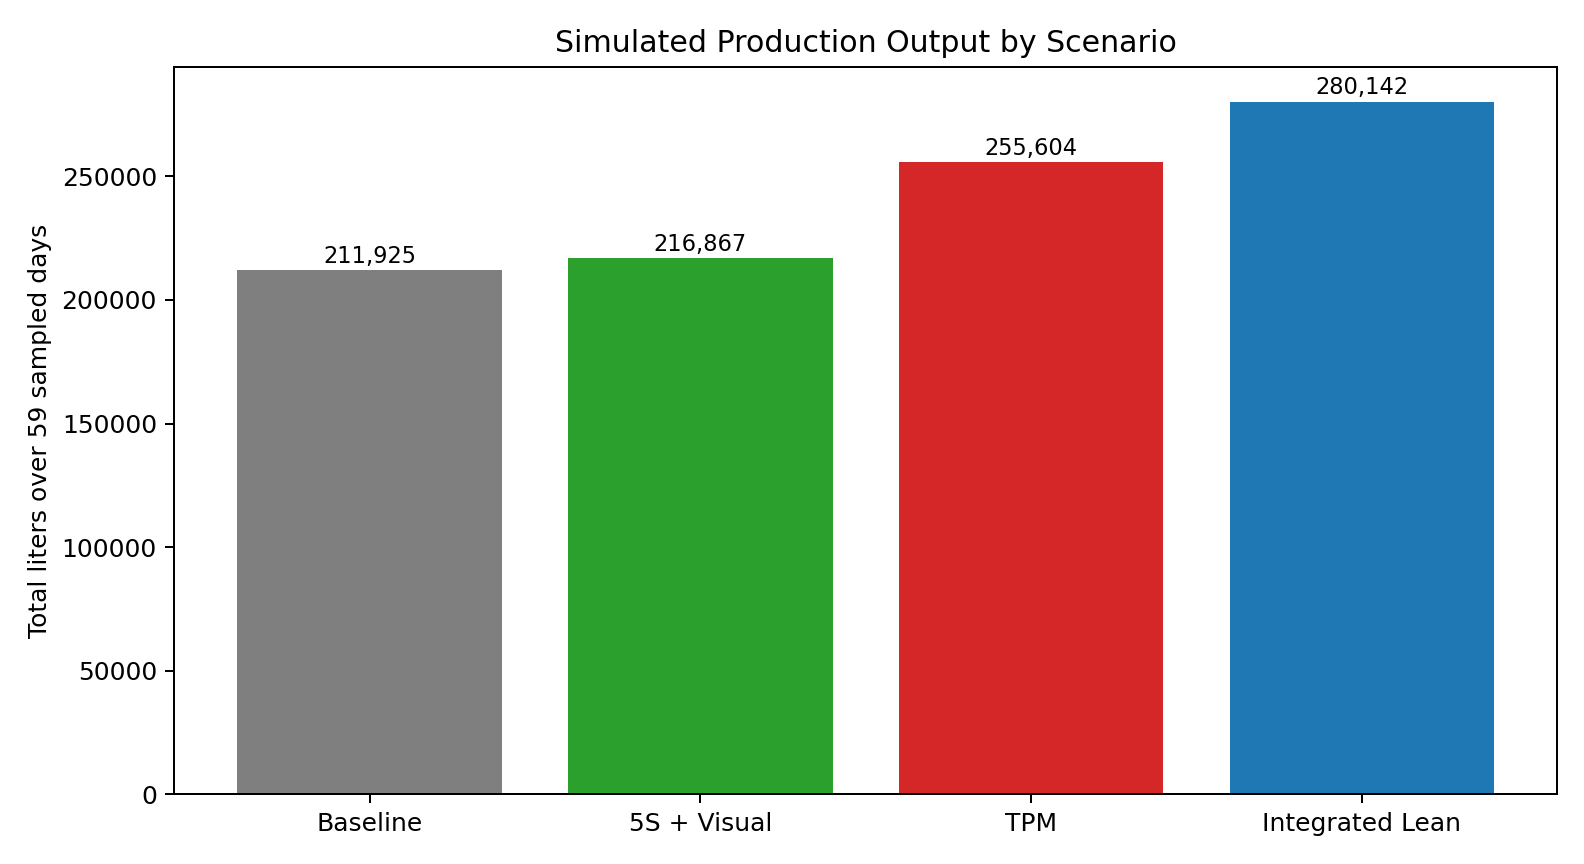
\includegraphics[width=\columnwidth]{outputs/scenario_output.png}
\caption{Mean simulated output across the baseline and lean scenarios.}
\end{figure}

The results show that 5S and visual management produce only a modest gain because they mainly address micro-stoppages. Total productive maintenance produces a much stronger gain because it targets the dominant lost-time source. The integrated lean bundle performs best because it reduces waste across all stoppage classes.

\section{Discussion}
The findings show that lean prioritization should be based on the structure of loss rather than the visibility of problems. In many factories, micro-stoppages are more visible because they happen frequently, but they may not be the dominant source of lost output. In the present case, major stoppages are the primary productivity driver.

This explains why TPM produces much larger gains than 5S alone. The result is consistent with the wider lean-simulation literature, which emphasizes context-sensitive tool selection [4], [5]. It also supports the argument that simulation is particularly valuable for SMEs, where incorrect prioritization is costly [3].

The study also strengthens the link between lean and digital manufacturing. Instead of relying only on static value stream mapping, the analysis uses event-level data, operational variability, and simulation. This is aligned with the direction suggested by smart manufacturing and digital twin research [6], [10].

\section{Conclusion}
This paper presented a self-contained IEEE-format study on simulation-based lean manufacturing using a real industrial beverage bottling dataset. The line suffers from low availability, large downtime, and strong variability over time. Although micro-stoppages are the most frequent events, major stoppages dominate total lost time.

The simulation showed that 5S and visual management improve output by 2.33\%, TPM improves output by 20.61\%, and an integrated lean bundle improves output by 32.19\% while raising simulated availability from 42.37\% to 55.33\%.

The main managerial implication is clear: maintenance-led reduction of major stoppages should be prioritized first, followed by workplace organization and broader stabilization efforts. The main academic contribution is a reproducible open-data framework for lean-simulation research suitable for final-year engineering work and SME-oriented manufacturing studies.

\section*{Acknowledgment}
The authors sincerely acknowledge the guidance and support of Dr.\ MOHD SHUAIB from the Mechanical Department. His guidance was valuable in shaping the direction and structure of this work.

\begin{thebibliography}{11}

\bibitem{r1}
I. Belekoukias, J. A. Garza-Reyes, and V. Kumar, ``The impact of lean methods and tools on the operational performance of manufacturing organisations,'' \emph{International Journal of Production Research}, vol. 52, no. 18, pp. 5346--5366, 2014, doi: 10.1080/00207543.2014.903348.

\bibitem{r2}
O. Oleghe and K. Salonitis, ``Hybrid simulation modelling of the human-production process interface in lean manufacturing systems,'' \emph{International Journal of Lean Six Sigma}, vol. 10, no. 2, pp. 665--690, 2019, doi: 10.1108/IJLSS-01-2018-0004.

\bibitem{r3}
F. Yu and Z. Chen, ``Tools, application areas and challenges of factory simulation in Small and Medium-Sized Enterprises -- A Review,'' \emph{Procedia CIRP}, vol. 104, pp. 399--404, 2021, doi: 10.1016/j.procir.2021.11.067.

\bibitem{r4}
J. Possik, A. Zouggar-Amrani, B. Vallespir, and G. Zacharewicz, ``Lean techniques impact evaluation methodology based on a co-simulation framework for manufacturing systems,'' \emph{International Journal of Computer Integrated Manufacturing}, vol. 35, no. 1, pp. 91--111, 2022, doi: 10.1080/0951192X.2021.1972468.

\bibitem{r5}
S. Frecassetti, B. Kassem, K. Kundu, M. Ferrazzi, and A. Portioli-Staudacher, ``Introducing Lean practices through simulation: A case study in an Italian SME,'' \emph{Quality Management Journal}, vol. 30, no. 2, pp. 90--104, 2023, doi: 10.1080/10686967.2023.2171326.

\bibitem{r6}
J. A. C. Bokhorst, W. Knol, J. Slomp, and T. Bortolotti, ``Assessing to what extent smart manufacturing builds on lean principles,'' \emph{International Journal of Production Economics}, vol. 253, art. no. 108599, 2022, doi: 10.1016/j.ijpe.2022.108599.

\bibitem{r7}
G. A. David, P. M. C. Monson, C. Soares Junior, P. O. Conceicao Junior, P. R. Aguiar, and A. Simeone, ``IoT-Driven Deep Learning for Enhanced Industrial Production Forecasting,'' \emph{IEEE Internet of Things Journal}, vol. 11, no. 23, pp. 38486--38495, 2024, doi: 10.1109/JIOT.2024.3447579.

\bibitem{r8}
G. A. David, P. M. C. Monson, and C. Soares Junior, \emph{Industrial Production Time-Series Dataset from a Beverage Bottling Line}. Zenodo, Jan. 4, 2026. doi: 10.5281/zenodo.18146866.

\bibitem{r9}
J. M. Matindana and M. J. Shoshiwa, ``Lean manufacturing implementation in food and beverage SMEs in Tanzania: using structural equation modelling (SEM),'' \emph{Management System Engineering}, vol. 4, no. 1, pp. 1--14, 2025, doi: 10.1007/s44176-025-00036-3.

\bibitem{r10}
M. Reslan, M. J. Triebe, R. Venketesh, and A. J. Hartwell, ``Automation of Value Stream Mapping: A Case Study on Enhancing Lean Manufacturing Tools Through Digital Twins,'' \emph{Procedia CIRP}, vol. 134, pp. 455--460, 2025, doi: 10.1016/j.procir.2025.02.159.

\bibitem{r11}
C. Unal and S. Bilget, ``Examination of lean manufacturing systems by simulation technique in apparel industry,'' \emph{The Journal of The Textile Institute}, vol. 112, no. 3, pp. 377--387, 2021, doi: 10.1080/00405000.2020.1756104.

\end{thebibliography}

\end{document}
